\documentclass[a4paper]{article}
\usepackage[margin=0.9in]{geometry}
\usepackage{graphicx}
\usepackage{float}
\usepackage{mathtools}
\usepackage{amsmath}
%\usepackage{subfigure}
\usepackage{color}
\usepackage[usenames,dvipsnames,svgnames,table]{xcolor}
\usepackage{amssymb}
\usepackage{pifont}
\usepackage[english]{babel}
\usepackage[hidelinks]{hyperref}
\usepackage{fancyvrb}
\usepackage{bera}
\usepackage{algorithm}
\usepackage{algorithmic}
\usepackage{caption}
\usepackage{subcaption}
\newcommand{\cmark}{\ding{51}}%
\newcommand{\xmark}{\ding{55}}%
\renewcommand{\algorithmicforall}{\textbf{for each}}
\usepackage[utf8]{inputenc}
\usepackage[english]{babel}
 
\setlength{\parindent}{0em}
\setlength{\parskip}{1em}

\usepackage{listings}
\usepackage{color} %red, green, blue, yellow, cyan, magenta, black, white
\definecolor{mygreen}{RGB}{28,172,0} % color values Red, Green, Blue
\definecolor{mylilas}{RGB}{170,55,241}
% Using typewriter font: \ttfamily inside \lstset
\lstset{language=Matlab,%
    %basicstyle=\color{red},
    breaklines=true,%
    morekeywords={matlab2tikz},
    keywordstyle=\color{blue},%
    morekeywords=[2]{1}, keywordstyle=[2]{\color{black}},
    identifierstyle=\color{black},%
    stringstyle=\color{mylilas},
    commentstyle=\color{mygreen},%
    showstringspaces=false,%without this there will be a symbol in the places where there is a space
    basicstyle=\small\ttfamily,
    %numbers=left,%
    numberstyle={\tiny \color{black}},% size of the numbers
    numbersep=9pt, % this defines how far the numbers are from the text
    tabsize=4,
    emph=[1]{for,end,break},emphstyle=[1]\color{red}, %some words to emphasise
    %emph=[2]{word1,word2}, emphstyle=[2]{style},    
}

\begin{document}
\title{Autonomous Robots Lab report \\ \#1 Potential Functions – Brushfire algorithm and
Wavefront planner}
\author{Kaisar Kushibar\\
Master of Computer VIsion and RoBOTics (ViBot)\\University of Girona (Girona)}

\maketitle
%------------------------------------

%\begin{abstract}
%This document is a report concerning the activities developed as laboratory for the discipline Probabilistic Robotics.
%\end{abstract}

\section{Introduction}
In this laboratory work we are going to study and implement two different potential function algorithms: Brushfire and Wavefront. We will explain in details the approaches that we used to accomplish the given tasks and also illustrate and discuss the obtained results.
\section{Potential functions}
Potential functions are very useful in obstacle avoidance and path planning. The main idea of this function is to provide information that allows to the robot to avoid obstacles, which have high potentials and move towards areas that have low potentials. The figure below illustrates an example of potential function.
\begin{figure}[H]
\centering
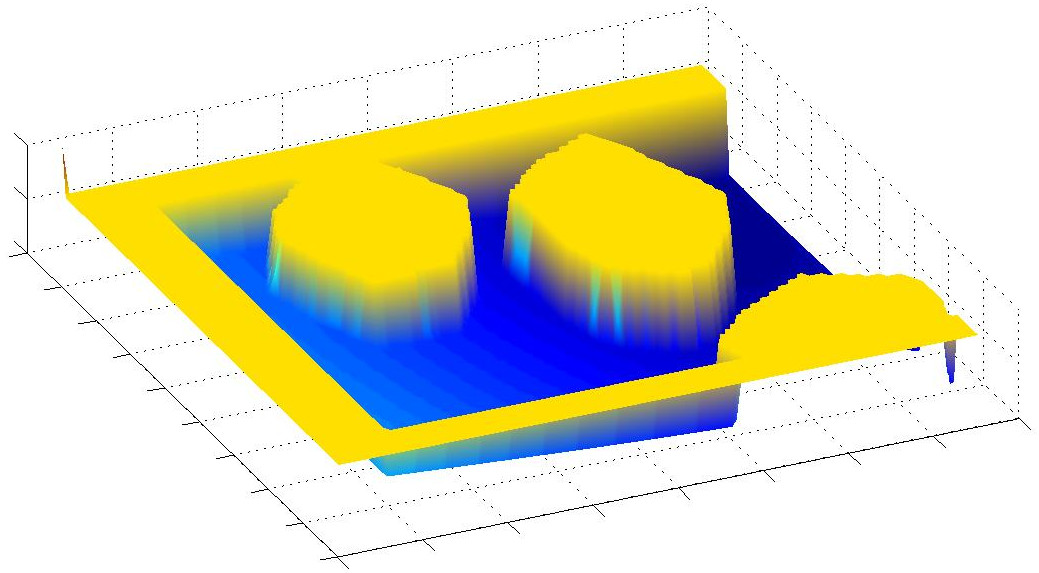
\includegraphics[width=3in]{potential-function}
\caption{Potential function example.}
\label{fig:potentialfunction}
\end{figure}
The obstacles have high potentials, which appear in yellow color in the Fig.~\ref{fig:potentialfunction}, whereas the low potential areas shown in blue. In order to apply this method it is required to know the map in advance and it is not adaptive for changes in the world. However, once the world is known, this method is very robust and useful to find an optimal path to the goal or define that the goal is not reachable.\\
In the following sections we are going to show the brushfire algorithm for generating potentials of repulsive obstacles and the wavefront planner for finding an optimal path from one point to another.
\section{Brushfire algorithm}
In this section we will show the approach that we used to implement the brushfire algorithm as well as the results we obtained.
\subsection*{Problem definition}
We are given a finite map - two dimensional matrix where the elements are equal to one if there is an obstacle and to zero otherwise. The goal is to fill the free areas with potential values  so that the areas that close to the walls and the obstacles will have the high potentials and the areas that far will have low potentials. Note that our implementation will generate a value map which is contrary to the definition, but it is easy to get a complement of the value map and obtain desired result.
\subsection*{Algorithm}
There exist several ways to implement this algorithm:
\begin{itemize}
\item Brute-force approach - for every element of the matrix try to find an adjacent cell that has a value and assign to the current element an increment of the value of its neighbour. This process should be repeated until all the cells of the map will have a value. This method is time consuming and not an efficient way, because it has to visit all the cells more than once.
\item Breadth first search (BFS) - considers having a queue structure which will contain elements that has to be visited. Initially the queue will have all the coordinates of walls and obstacles. At each step we look at the adjacent pixels of the first element from the queue and if they have no value we assign them a value and add it to the queue. Then, remove the current pixel and repeat the process. Using this method we visit every cell only once and therefore it takes less time to fill the whole map.
\end{itemize}
For the brushfire algorithm we used BFS method and the pseudo-code of our implementation is given below.
\begin{algorithm}[H]
\caption{Brushfire algorithm}
\label{brushfireAlgo}
\begin{algorithmic}[1]
\STATE INITIALIZE $queue$ = wall and obstacle cells
\WHILE{$queue$ is not empty}
\STATE $p$ = first element of $queue$
\FORALL{$adjacentCell$ of $p$}
\IF{$ValueOf(adjacentCell)$ is $0$}
\STATE $ValueOf(adjacentCell)$ $\Leftarrow$ $ValueOf(p) + 1$
\STATE $queue$ $\Leftarrow$ $adjacentCell$
\ENDIF
\ENDFOR
\STATE remove $p$ from $queue$
\ENDWHILE
\end{algorithmic}
\end{algorithm}

\subsection*{Results}
In this section we illustrate results that we obtained with our implementation. In all figures black areas represent obstacles and walls.

\begin{figure}[H]
\centering
	\begin{subfigure}[t]{3in}
		\centering
		
\includegraphics[height=2.3in]{bf-simple}
		\caption{Size: 14x20; Time: 0.000158 seconds}\label{fig:bf-a}
	\end{subfigure}
	\quad
	\begin{subfigure}[t]{3in}
		\centering
		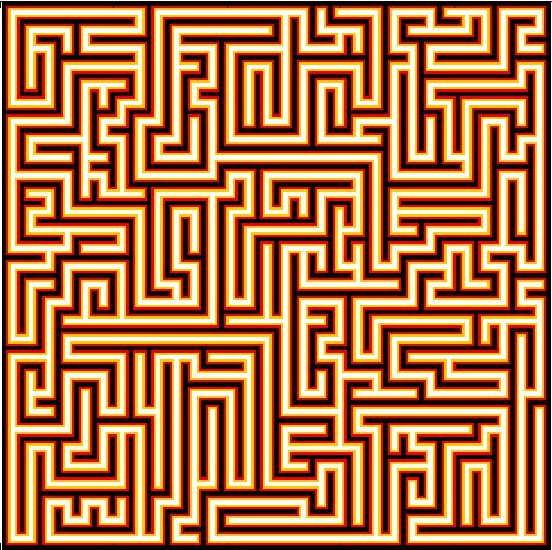
\includegraphics[height=2.3in]{bf-maze}
		\caption{Size: 242x242; Time: 0.020723 seconds}\label{fig:bf-b}
	\end{subfigure}
	\quad
	\begin{subfigure}[t]{3in}
		\centering
		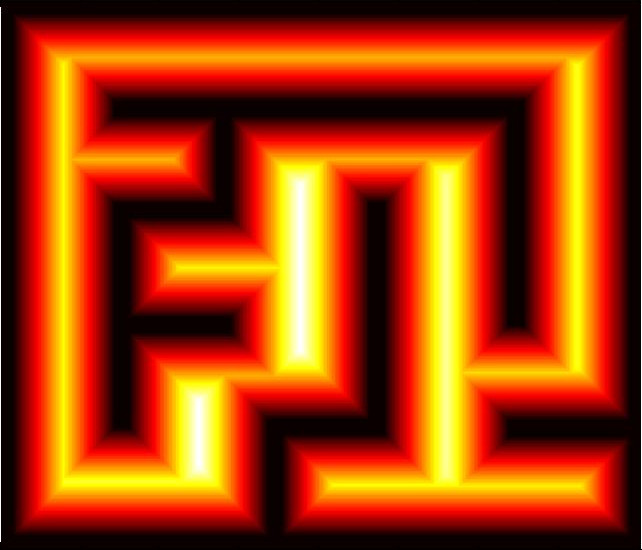
\includegraphics[height=2.3in]{bf-mazeBig}
		\caption{Size: 687x802; Time: 0.171600 seconds}\label{fig:bf-c}
	\end{subfigure}
	\quad
	\begin{subfigure}[t]{3in}
		\centering
		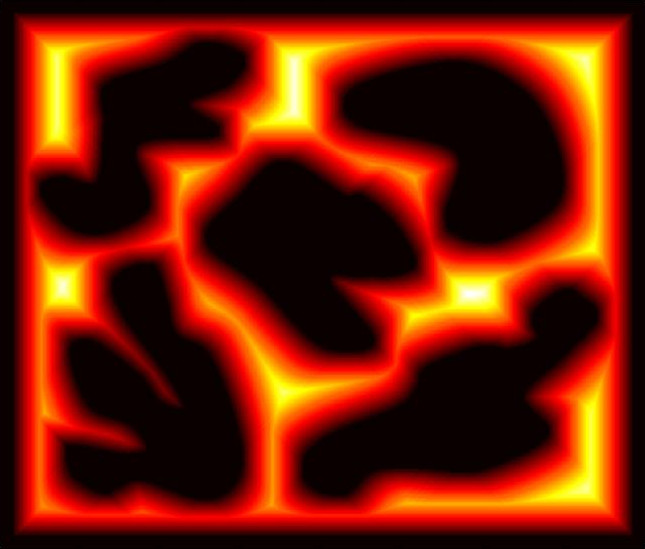
\includegraphics[height=2.3in]{bf-obstaclesBig}
		\caption{Size: 683x803; Time: 0.185738 seconds}\label{fig:bf-d}
	\end{subfigure}
\caption{Brushfire algorithm results.}
\label{fig:bf-map}
\end{figure}

From the results it can be seen that using BFS algorithm with a queue structure gives a high performance.

\section{Wavefront planner}
Wavefront planner algorithm consist of two steps: (1) generating a value map; (2) finding the shortest path using the value map from starting point to the goal point.
\subsection*{Value map construction}
The first part of the algorithm is very similar to the brushfire method, but instead of generating repulsive potential map it spreads a wave starting from one cell (e.g. goal point) until it covers all the field. Every cell (excluding walls and obstacles) in the resulting value map represents the shortest path from the initial position to that cell. If one cell has a value equal to zero, then it means that cell is impossible to reach from the starting position. This part is also implemented using BFS algorithm (Algorithm~\ref{brushfireAlgo}) with only one change: the queue is initialized with the goal point instead of obstacles (line 1).\\
The figure-set below illustrates how the wave is spread from the starting position (top-right) and filled all the area flowing around the obstacles.
\begin{figure}[H]
\centering
\begin{subfigure}[t]{3in}
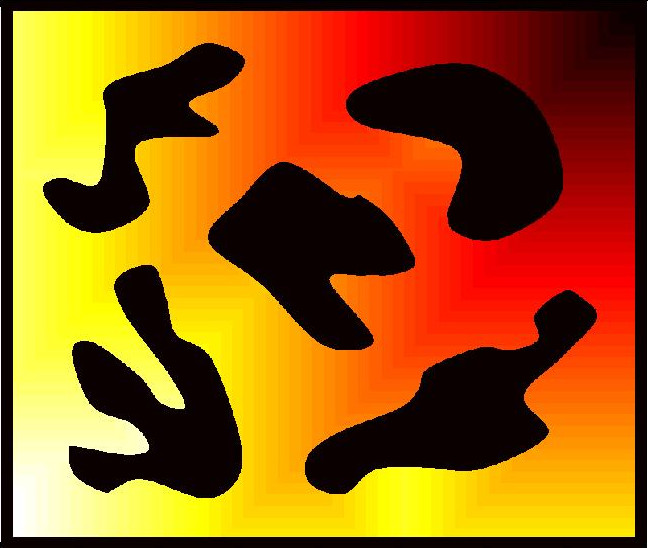
\includegraphics[width=3in]{wf-val-obstBig}
\end{subfigure}
\begin{subfigure}[t]{3in}
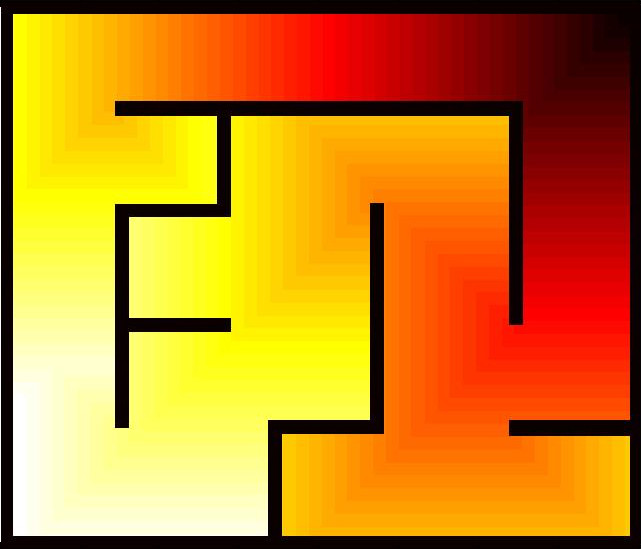
\includegraphics[width=3in]{wf-val-mazeBig}
\end{subfigure}
\caption{Value map of wavefront algorithm.}
\label{fig:wf-val-obstBig}
\end{figure}

\subsection*{Finding a trajectory}
In this part we will show our approach in finding a shortest path from the starting point to the goal. As we said before, the value of a cell after value map construction represents the distance from the starting point to that cell. Accordingly the adjacent points to that cell contain the same information, but their values may differ if they are located closer or farther from the starting point. Using this property we will try to build a path by following the values in a descending order until we reach to the minimum (i.e. starting point). The important part that we have to consider is that going vertical or horizontal is preferable rather than going diagonal. Following diagonal path may cause oscillating path, which is not optimal if we consider the euclidean distance. The pseudo-code below shows our implementation of optimal trajectory finding algorithm.

\begin{algorithm}[H]
\caption{Optimal path finding algorithm}
\label{wfAlgo}
\begin{algorithmic}[1]
\STATE INITIALIZE $trajectory$ = $start$
\STATE INITIALIZE $currentCell$ = $start$
\REPEAT
\FORALL{$adjacentDiagonalCell$ of $currentCell$}
\IF{$ValueOf(adjacentDiagonalCell)$ < $ValueOf(currentCell)$}
\STATE $candidateCell$ $\leftarrow$ $adjacentDiagonalCell$
\ENDIF
\ENDFOR
\FORALL{$adjacentCell$ of $currentCell$}
\IF{$ValueOf(adjacentCell)$ < $ValueOf(currentCell)$}
\STATE $candidateCell$ $\leftarrow$ $adjacentCell$
\ENDIF
\ENDFOR
\STATE put $candidateCell$ to $trajectory$
\STATE $currentCell$ $\leftarrow$ $candidateCell$
\UNTIL{$currentCell$ is not $goal$}
\end{algorithmic}
\end{algorithm}

\subsection*{Results}
The figure-set below illustrates the results of trajectory finding algorithm. The trajectory is shown in white.
\begin{figure}[H]
\centering
	\begin{subfigure}[t]{3in}
		\centering
		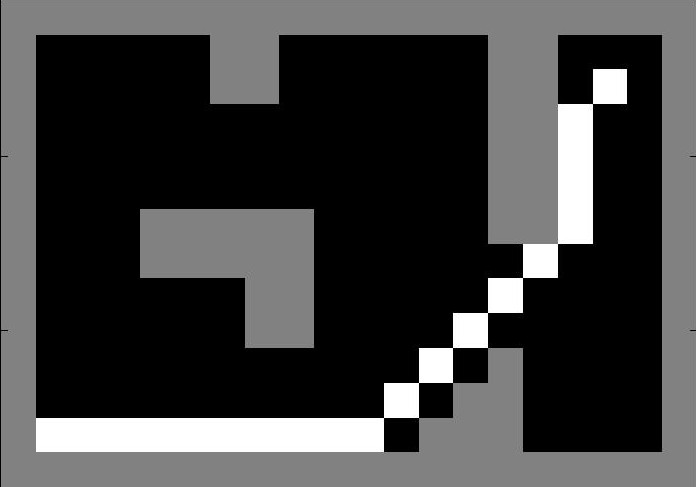
\includegraphics[height=2.3in]{wf-simple}
		\caption{Size: 14x20; Time: 0.000109 seconds}\label{fig:wf-a}
	\end{subfigure}
	\quad
	\begin{subfigure}[t]{3in}
		\centering
		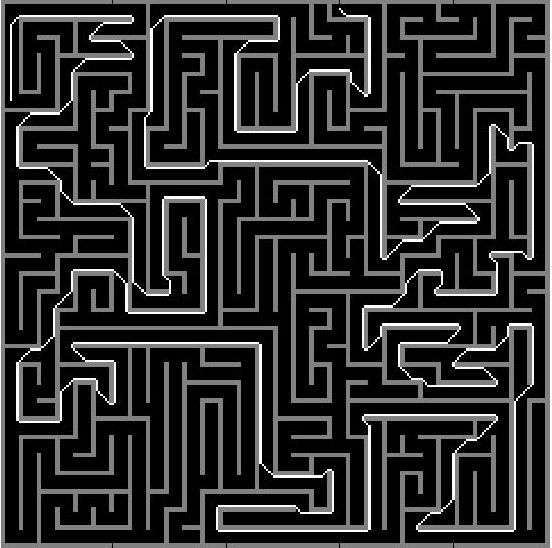
\includegraphics[height=2.3in]{wf-maze}
		\caption{Size: 242x242; Time: 0.027039 seconds}\label{fig:wf-b}
	\end{subfigure}
	\quad
	\begin{subfigure}[t]{3in}
		\centering
		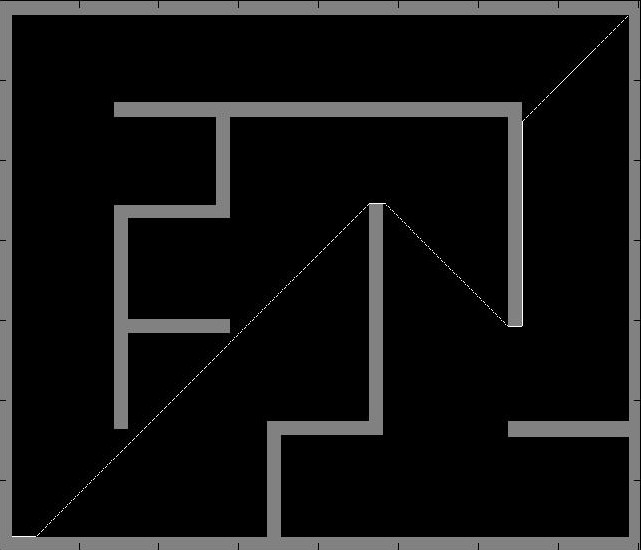
\includegraphics[height=2.3in]{wf-mazeBig}
		\caption{Size: 687x802; Time: 0.100510 seconds}\label{fig:wf-c}
	\end{subfigure}
	\quad
	\begin{subfigure}[t]{3in}
		\centering
		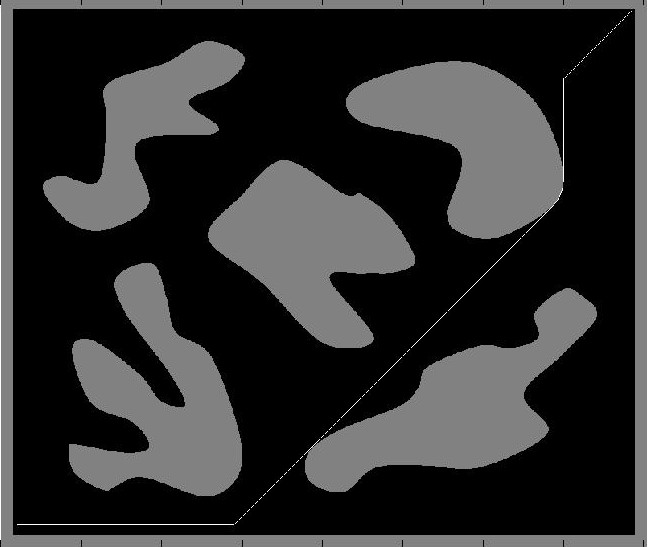
\includegraphics[height=2.3in]{wf-obstaclesBig}
		\caption{Size: 683x803; Time: 0.097116 seconds}\label{fig:wf-d}
	\end{subfigure}
\caption{Wavefront planner results. Computation time is shown including value map construction and trajectory finding parts.}
\label{fig:bf-map}
\end{figure}

\section{Conclusion}
In this laboratory work we studied two potential function algorithms: brushfire and wavefront. We used brushfire algorithm to build repulsive potential map and wavefront for planning a path from one point to another. We implemented these algorithms and tested with different maps. We also discussed algorithm and implementation details including their performances. Finally, we illustrated the obtained results of different maps and compared the computational time. This practice work helped us to better understand the topic and solidify our knowledge in potential functions.
\end{document}